\documentclass[runningheads,a4paper]{llncs}

\usepackage[utf8]{inputenc}


\usepackage[compatibility=false]{caption}
\usepackage{subcaption}

\usepackage{natbib}
\bibliographystyle{apalike-fr}

\usepackage{amssymb}
\setcounter{tocdepth}{3}
\usepackage{graphicx}% http://ctan.org/pkg/graphicx
\usepackage{array}% http://ctan.org/pkg/array

\usepackage[english]{babel}
\usepackage[T1]{fontenc}

\makeatletter
\newcommand{\@chapapp}{\relax}%
\makeatother

\usepackage[title,toc,titletoc,header]{appendix}


\begin{document}

\mainmatter 

\title{Neodroid: Simulation Environment And Interfaces}

\titlerunning{Neodroid: Simulation Environment And Interfaces}

\author{Christian Heider Nielsen}

\institute{SINTEF Ocean}

\authorrunning{Christian Heider Nielsen}

\maketitle

\begin{abstract}
This document serves as documentation for the Neodroid simulation environment and interfaces. The purpose of the implemented environment is a enable compilation of data sets to be utilised for training machine learning models. It comprises a specific simulation of a parallel jaw gripper navigating a difficult environment and grasping fish-like objects, throughout the simulation RGB images, Depth images, positions and rotations are recorded. The Neodroid interface strives to aid a researcher in rapidly developing new simulation environments for reinforcement learning tasks. One component of the interface system serves purposely restricted information about, and access to excitable motors, within the running simulation environment. While another component enables communication to the running environment, as simple method calls on python objects. The interface system presents some abstractions designed to quickly develop a general mental model for simulation environment at hand. 
\end{abstract}

\vspace{\fill}

\begin{figure}
\centering

\includegraphics[height=1cm]{figures/sintef-header}
\end{figure}

\clearpage

\begingroup
\let\clearpage\relax
\tableofcontents
\endgroup

\clearpage

\section{Introduction}

%Imagine learning to perform any arbitrary simple task, like classifying a photograph as cat or not with knowing what a cat even is beforehand, by trying to correctly solve it repeatedly, over and over and over but every time on a completely new image of either a cat or not a cat. Failure to answer correctly will be punished. Moderate progress is made with each repetition as features such as whiskers, tails, ears, claws and texture are learned to be useful for correctly solving this task. There is a catch to learning in this manor, as it requires the examples of cat and not cats and someone that knows what a cat is has make these examples in the first place, , luckily internet search engines are around for us humans. Now take a much more complex task of correctly navigating a difficult three dimensional environment and picking an object with an robot arm, learning in the same fashion as the previously mentioned

%Physical robots suffer from the limitation of not being able to overcome physical constants of our universe as heat di, where as robots in simulated environment. 


Current state of the art in game engine, virtual reality and user-friendly development technologies allows for rapid prototyping of convincing environments, where in user can intuitively move around interact with objects. The Neodroid project strives to learn the user's intent from the user interacting with the environment. Once the intent is captured, a series of slightly differing simulations with the same intent can accelerate data collection, rather than the user tirelessly having to complete same intent repeatedly in only slightly differing environments. 
Once an agent has learned to replicate the intelligent behaviour and intent of the user through the use of the simulated data, it can explorer other possibly more efficient solution in a reinforcement learning environment.

As the first steps of the Neodroid project to achieve this intended behaviour, an initial problem of navigating and grasping a fish-like object is posed as means of trying to replicate a user's intent, see fig.~\ref{fig:problem-environment} for what the problem includes. One of these first steps is a scripted simulation emulate an user performing such task, in the simulation a gripper will find an unobstructed path through a some obstacles to a fish-like object, this will be described in section~\ref{sec:simulation}. Next step is the reinforcement learning environment, in section~\ref{sec:learning} a detailed description of the concepts and abstraction of the interface will be given.

\begin{figure}
\centering
\begin{subfigure}[t]{0.33\textwidth}
\centering
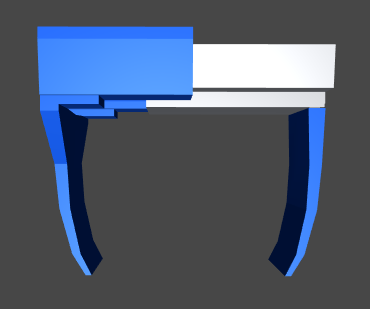
\includegraphics[width=\linewidth]{figures/gripper}
\caption{gripper}
\label{fig:gripper-sim}
\end{subfigure}%
    \hfill
\begin{subfigure}[t]{0.33\textwidth}
\centering
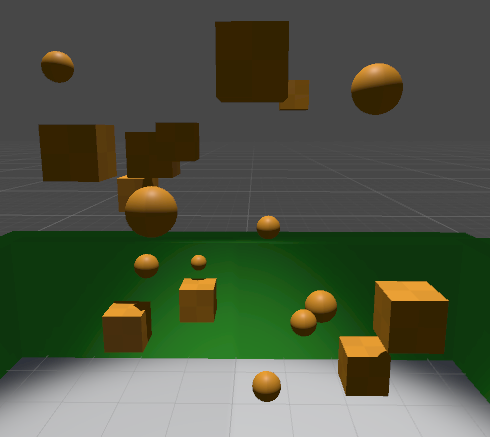
\includegraphics[width=\linewidth]{figures/obstructions}
\caption{obstructions}
\label{fig:obstructions-sim}
\end{subfigure}%
    \hfill
\begin{subfigure}[t]{0.33\textwidth}
\centering
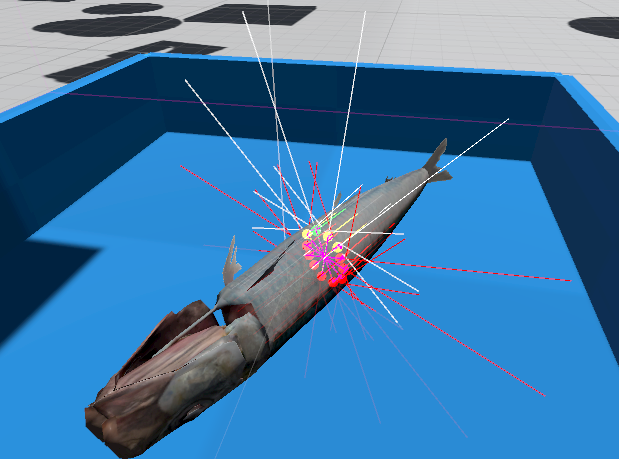
\includegraphics[width=\linewidth]{figures/target}
\caption{fish}
\label{fig:fish-sim}
\end{subfigure}%

\caption{In the problem enviroment 
(a) %\ref{fig:gripper-sim}
is the gripper that navigate the obstruction 
(b) %\ref{fig:obstructions} 
to the target fish 
(c)%\ref{fig:fish-sim}
.}
\label{fig:problem-environment}
\end{figure}

All material produced during the summer of 2017 for the Neodroid project is hosted at \url{https://github.com/sintefneodroid}, the source code is published under Apache License 2.0.

\section{Fish Grasping Simulation}\label{sec:simulation}

Supervised learning techniques requires a substantial amount of data to learn generalised functions for utilisation on unseen examples in any environment. The rate at which we can acquire such data in the our world is limited by time and physical constants of the universe we live in, furthermore this form of acquisition may also be costly financially. We can circumvent these limitations by carrying out precise simulations emulating the physical properties of our world. The precision of the simulation is key when any model trained on the simulated data, is applied on the data from the true distribution $p_{data}(X)$ the simulation was trying to emulate. This shift in the input data is coined domain transfer, in that the model is utilised in another domain than it was trained in. Failure to achieve sufficient precision in the simulations will most likely unexpected and unwanted behaviour by the agent using the model.[Find example]. 

Having the ability to control and observe every parameter in a simulation environment means that we can certainty rely on the observed state of the environment. This eases the development of domain specific and somewhat intelligent programs that carry perfectly carry out a intended task, this allows any observer to try learn from experts with fully observable state and seek out important cues that help with the task at hand.   

With importance of transferability of domain in mind we should sought to make the simulation as precise as is computationally feasible.

\cite{Dyrstad2016} constructed such simulations to allow models to learn how to detect and grasp objects in an environments but not to navigate the environment or approach grasp position and orientation. The contribution of this simulation environment quintessentially will take part in is the to allow machine learning model to learn programs from the scripted data in simulated environments, to then post training being applied in our world environment.

Screenshots from the simulation in action can be seen in appendix~\ref{app:simulation}.

\subsection{States}\label{sec:states}

The scripted behaviour is implemented with state machines, observing and registering events in the environment and then acting accordingly.

\begin{figure}
\centering
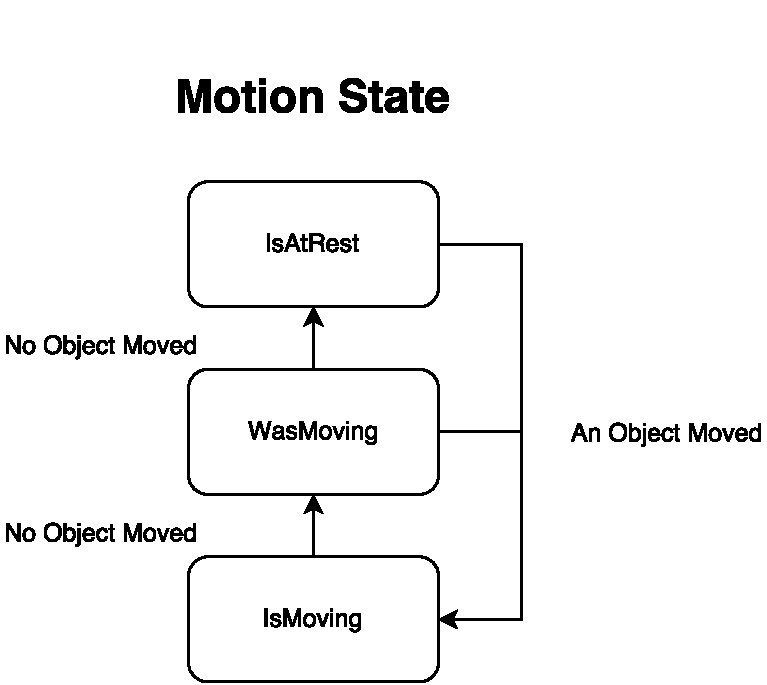
\includegraphics[width=.4\linewidth]{figures/statediagrams/motion-states.pdf}
\caption{motion-states}
\label{fig:motion-states}
\end{figure}

We want to know whether the current path we are following, is still valid or a collision might be occurring with an obstuction on the current course. Should it be the case that is not valid anymore, then we would want to recalculate and plan a new collision free course for the newly changed environment. The state machine depicted in fig.~\ref{fig:motion-states} is responsible for keeping track of this.

Similarly when a possible target object changes its orientation or location/position in the environment, we would want to recalculate the path and valid grasp or possibly even reconsider which target to pick up. It is implemented using the same state machine as depicted in fig.~\ref{fig:motion-states} but is tracking target instead of obstructions in the environment.

We could recalculate the target object and path on every frame, but as some noticeable time may sometimes be spend calculating such path in a difficult environment, we only want to recalculate when the environment changes and it is necessary.

\begin{figure}
\centering
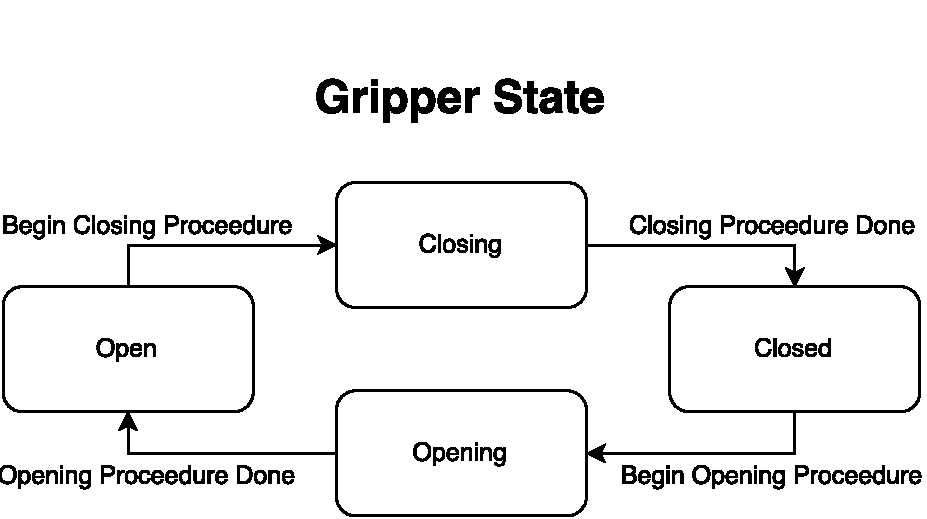
\includegraphics[width=.6\linewidth]{figures/statediagrams/gripper.pdf}
\caption{gripper}
\label{fig:gripper}
\end{figure}

Throughout the simulation we would want to track whether the grippers claw is in an open or closed position. Note that the simulation runs in discrete time steps which means that the gripper can be closing to reach a closed state or opening to an open state, leading to the gripper having 4 possible states, open, opening, closed and closing. Another way to track this was with a percentage but because the closed state position is not a fixed but in fact is dependent on the orientation, position and size of the target object the gripper is picking up, then a simpler two static state solution was chosen, depicted in fig.~\ref{fig:gripper}.

\begin{figure}
\centering
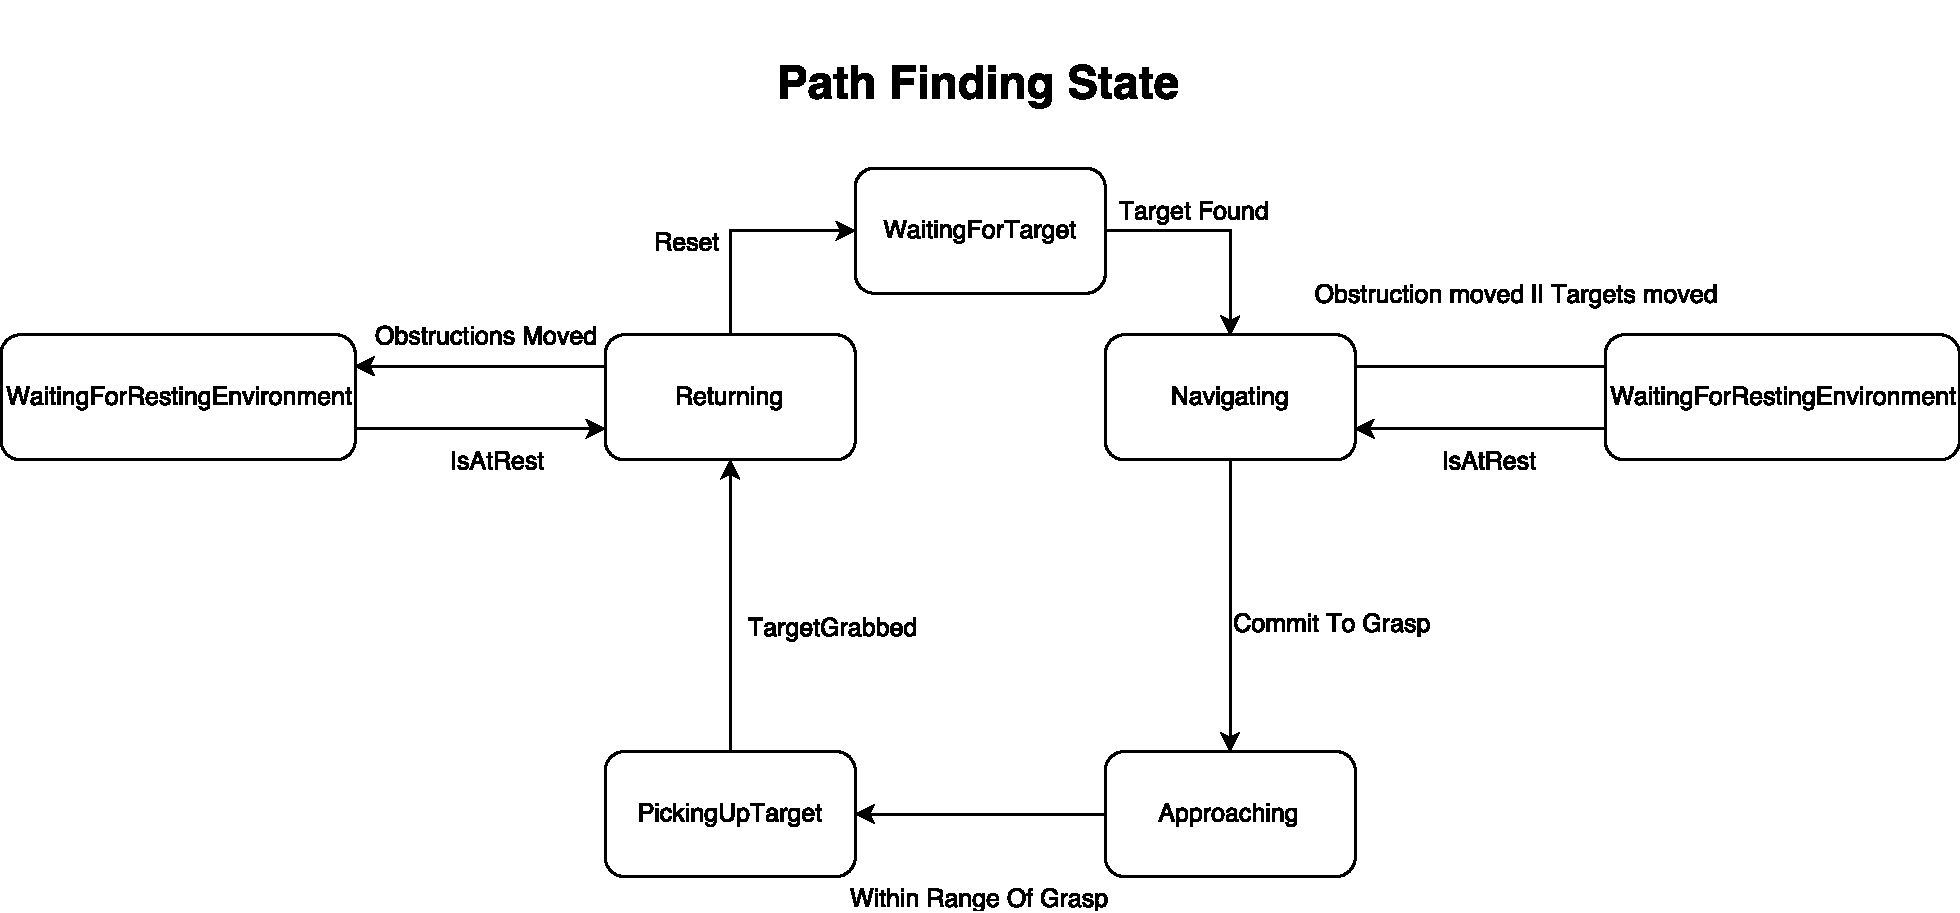
\includegraphics[width=\linewidth]{figures/statediagrams/path.pdf}
\caption{path}
\label{fig:path}
\end{figure}

Along the planned path the gripper is following, the gripper transitions through a number of phases that changes its behaviour slightly, like not rotating according to the targets orientation anymore or waiting for the environment to be at rest before continuing. fig.~\ref{fig:path} shows these states or phases if you will.

\begin{figure}
\centering
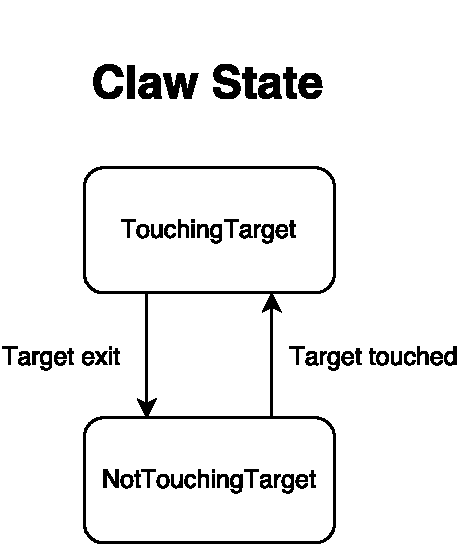
\includegraphics[width=.3\linewidth]{figures/statediagrams/claw-states.pdf}
\caption{claw states}
\label{fig:claw}
\end{figure}

Both claws of the gripper can possibly interacting the target, by touching it and thereby also be able to affect the target's position and orientation. The two states for each claw help to indicate whether or not we belief that we have a secure grasp around the object we are picking up. If the target is only touching one claw it is possible that the object, in this case fish, will just slip out of the gripper during pick up procedure or return procedure, fig.~\ref{fig:claw} depicts the states for these claws.

\begin{figure}
\centering
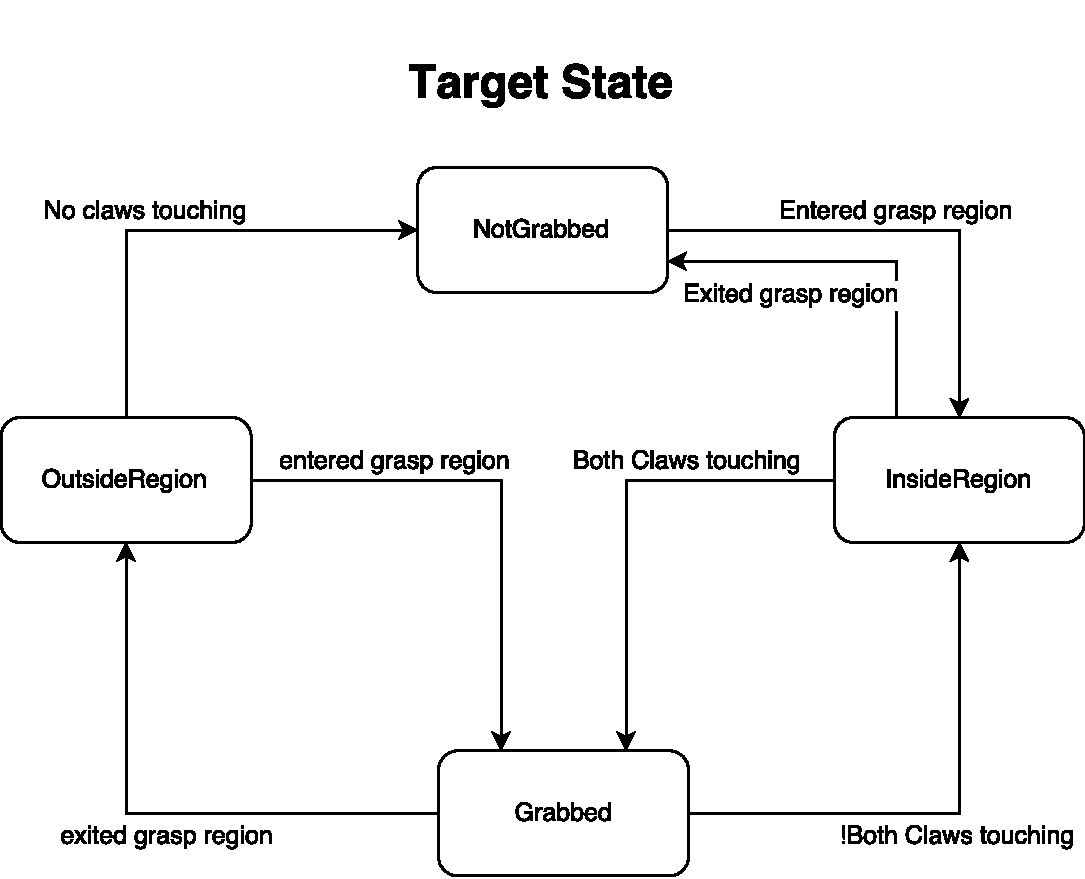
\includegraphics[width=.8\linewidth]{figures/statediagrams/target.pdf}
\caption{target}
\label{fig:target}
\end{figure}

The state machine depicted in fig.~\ref{fig:target}, tries to capture our current belief of the state of the target being picked up, it is possible that we lose the target during travel to destination or that we fail to pick it up in the first place. When picking up the target we are tracking whether the target is inside the region of the gripper where we expect a secure grasp, when this is the case we can change the state of the gripper to closing, which in turns closes claws and secures the target in place in the gripper.

\subsection{Usage Guide}

This section will briefly describe how to use the neodroid simulation.

The source code for the simulation environment is hosted at \url{https://github.com/sintefneodroid/simulation}.

\subsection{Issues}

The environment has some issues that degrades the realism of the simulation. 

\subsubsection{Shadows}

Calculating how each discrete point in the environment should be lighted is computationally extensive when trying to emulate how lighting in our world behaves, surfaces can be reflexive, luminant and the might be multiple light sources. Some assumptions and short comings is required to make rendering rate fast and smooth, this leads to limitations in what level of realism, we can achieve. In \cite{unity3d} each light source has shadow map with some fixed resolution according to the quality setting and the amount available ram on the gpu \cite{unityshadowmapsize}, this means if the light map span a larger area the pixelation is the shadows projected into the scene than when the light span a smaller area but keeps the same fixed resolution. Note that is the span is both affected by the distance the light source is from the projected surface and the field the light source spans in degrees. Section ~\ref{sec:shadowsexperiment} will explorer this issue further.

\subsubsection{Friction}

As of now friction between the target and the gripper relies on \cite{unityphysics} physics system, which is imprecise at best. To keep the target relatively stable within the jaws of the gripper, the target object is applied the same forces at the gripper additional to any gravitational or velocity forces affecting the target. It is important to note that these forces would be preferred to be affecting the target indirectly through the proxy colliders on the grippers jaws, but this is not the case as the \cite{unity3d} physics system is not precise enough and simply cant approximate this intented behaviour.

\subsubsection{Colliders}

One issue with the current simulation is when the object to be picked up has more than one collider interconnected via joint, then the \cite{unityphysics} physics system ends up in a unstable simulation and causes quite unpredictable and nonsensical undesired behaviour, the individual colliders of the fish-like object chaotically collides with the gripper while constantly trying the keep up the maximum angle of the joints until twisting the object out the grasp of the gripper.

\section{Reinforcement Learning Interface}\label{sec:learning}

This section will present an interface for use in a reinforcement learning context.
The interface should reflect experiments executed in our universe and therefore should only present information to the agent that realistic acquisitional in our universe, this is to intentionally limit what of the observable state is that is directly exposed the agent.

The interface is heavily inspired by the reinforcement learning toolkit from \cite{openai}. The agent start off by connecting to the environment and receives the initial state of the environment. Now at each discrete time of the simulation the must decide on how to react to the current state of the environment. Then after execution of the reaction a new state which includes a reward for the previous step is returned for agent to reaction upon again. This loop is depicted fig.~\ref{fig:loop}. This loop continues until termination on either side, agent or simulation.

\begin{figure}
\centering
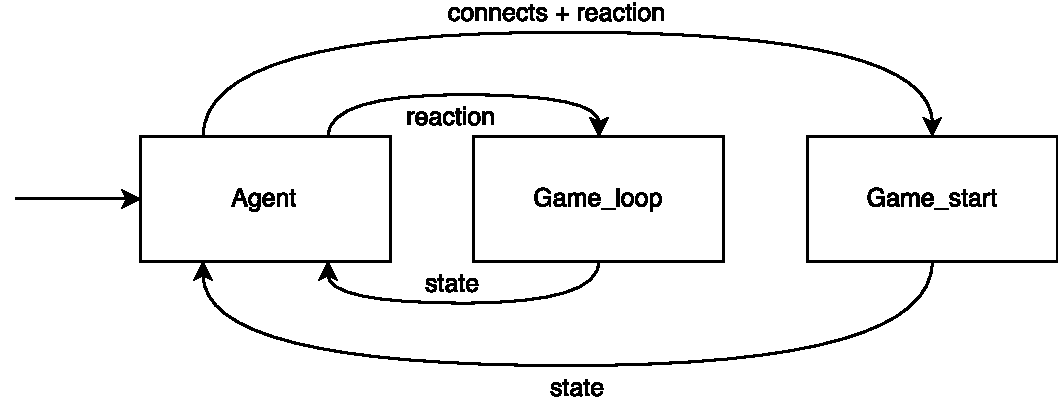
\includegraphics[width=.6\linewidth]{figures/neodroid_agent_game.pdf}
\caption{The agent-simulation loop}
\label{fig:loop}
\end{figure}

The loop under the hood is modelled with a request socket and a corresponding response, which can easily be thought off as being respectively a client and a server in a client-server architecture. The simulation(server) waits for an agent(client) to connect and somehow mutate the state of the simulation, see fig.~\ref{fig:networking} for a visual depiction.

\begin{figure}
\centering
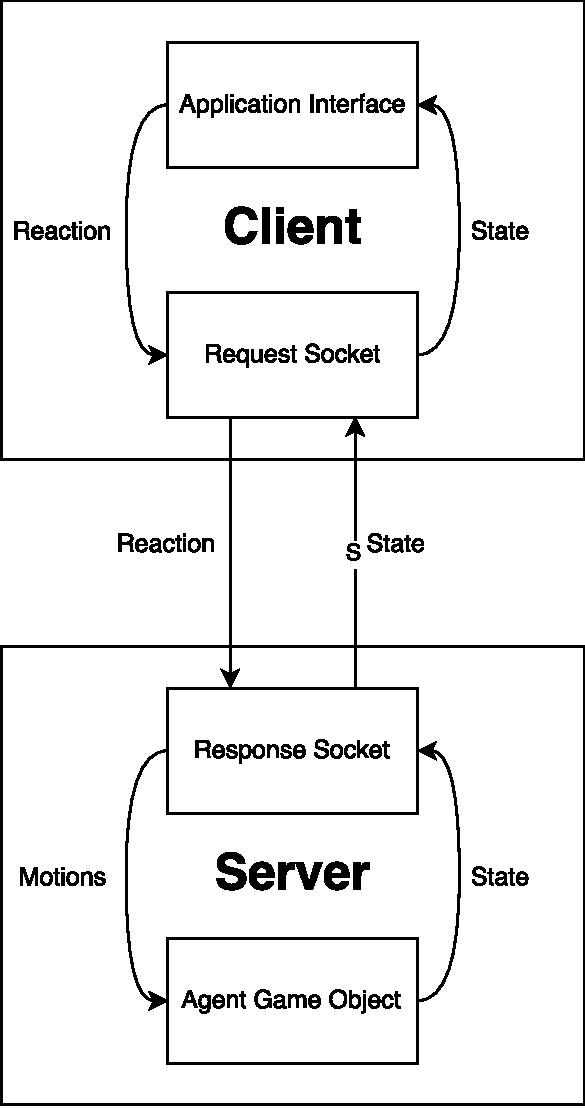
\includegraphics[width=.3\linewidth]{figures/networking.pdf}
\caption{The agent-simulation loop in a networking perspective}
\label{fig:networking}
\end{figure}

\subsection{Models}

In design of the interface some effort was made to build a intuitional mental model for thinking about the environments the agents with be interacting with, fig.~\ref{fig:interaction} is the result  of that effort. Each connection from one entity to another denotes an interactions between these, the direction denotes whether the entity is influenced by or influences the other entity.

\begin{figure}
\centering
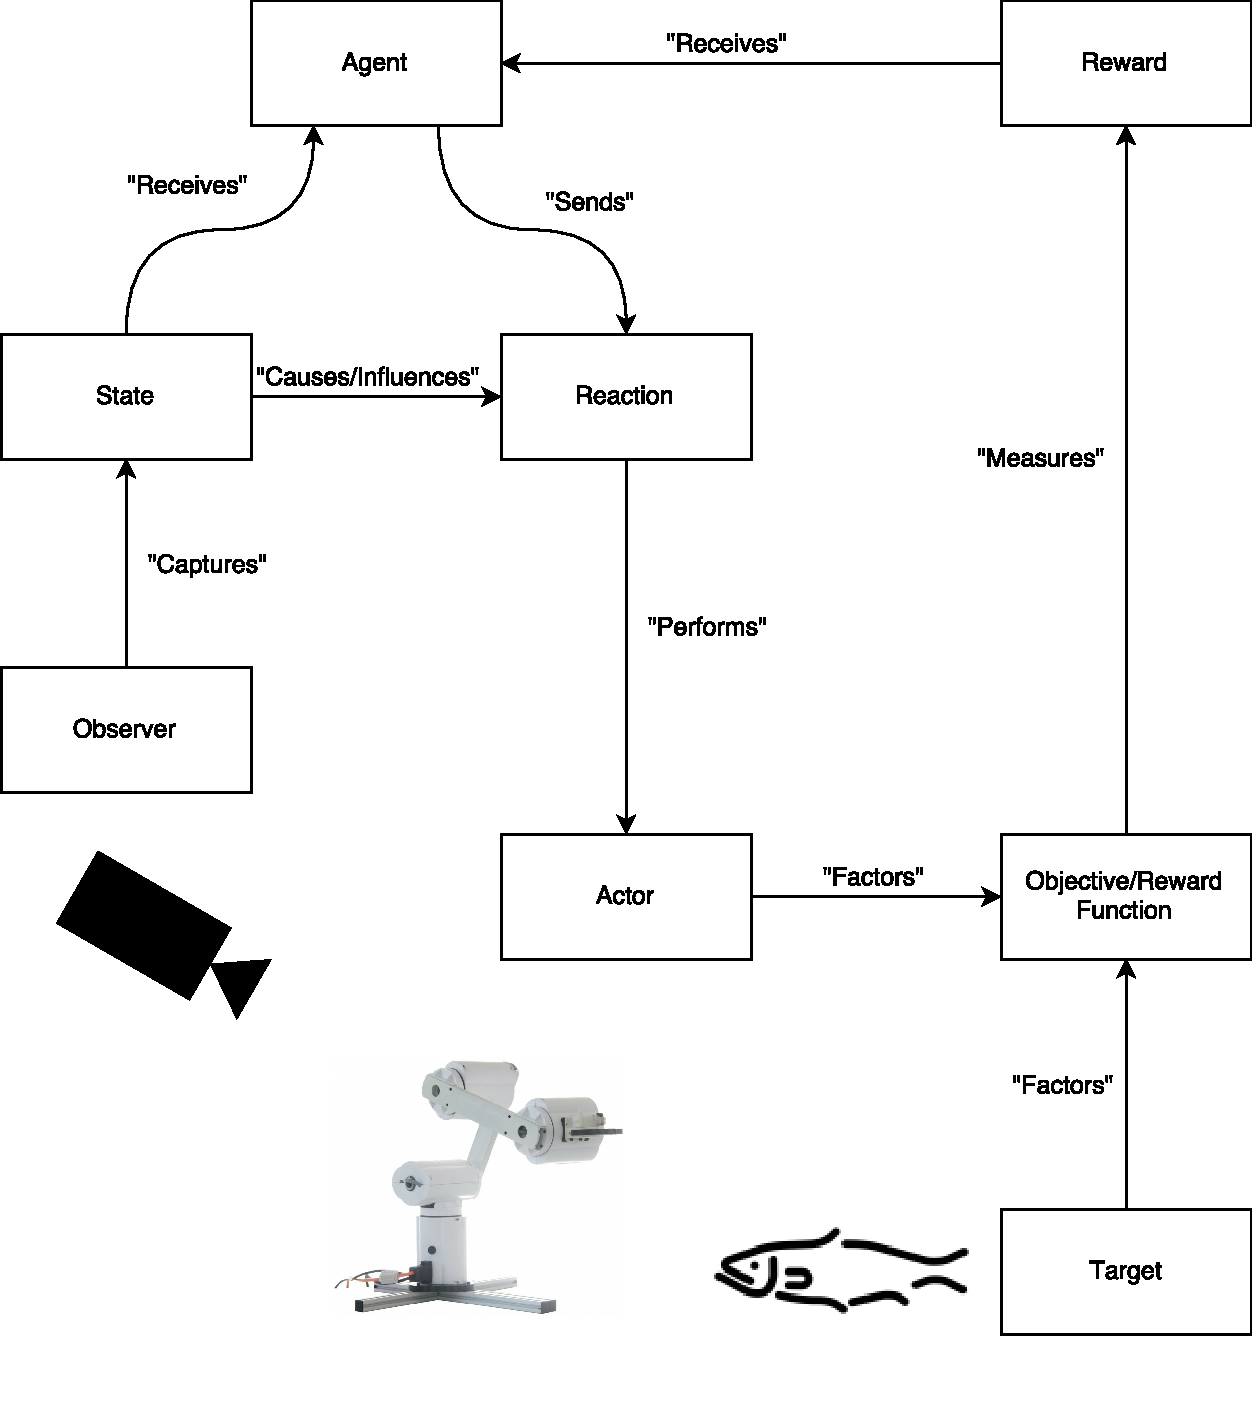
\includegraphics[width=.9\linewidth]{figures/neodroid_classes_verbs.pdf}
\caption{Interaction of models in the Neodroid interface}
\label{fig:interaction}
\end{figure}

Fig.~\ref{fig:classes} is the formalised classes of the earlier interaction activity. Following will be conceptual descriptions of each of the formalised classes.

\begin{figure}
\centering
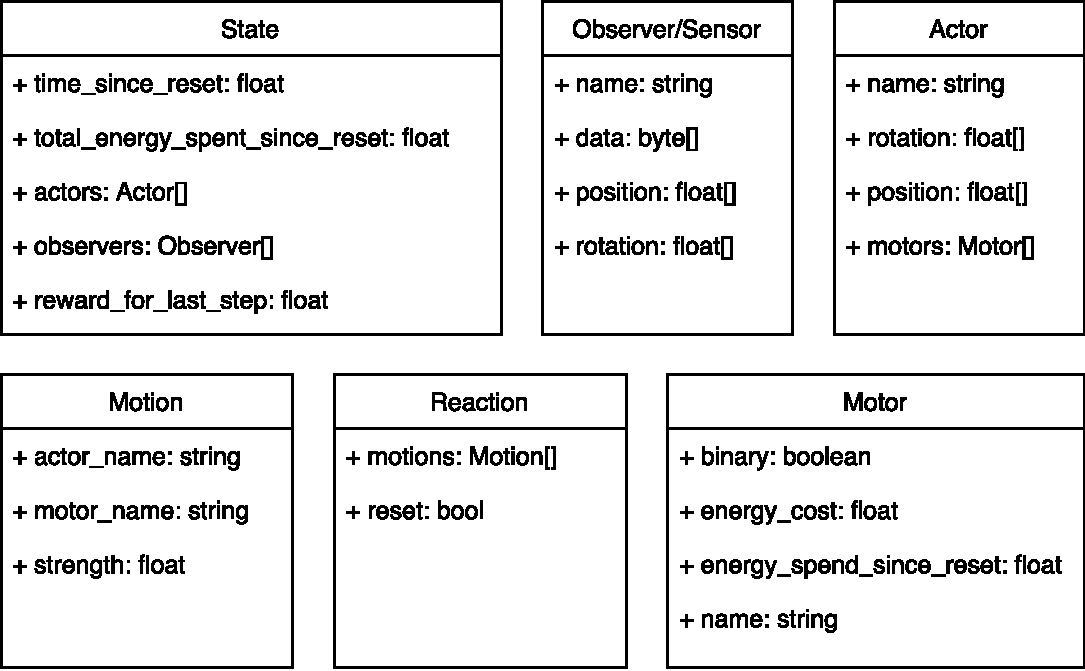
\includegraphics[width=.8\linewidth]{figures/neodroid_classes.pdf}
\caption{Classes of the Neodroid interface}
\label{fig:classes}
\end{figure}

\subsubsection{Actor}

The concept of the actor model is that is that is encapsulates a number of motors as part of one entity. For example as brushless electric motors on a multirotor aircraft, here the actor is the aircraft and the motors in are the brushless electric motors.

\subsubsection{Agent}

The agent model is an abstraction of some external agent providing reactions to be acted out in the environment. The agent abstraction has the responsibility of providing the interface for external agents into the environment, this include passing messages back and forth through a TCP connection or likewise. 

\subsubsection{Environment State}

The environment state encapsulates all information that should be exposed to external agents into one message. This message is comprised of observers  with their relevant observational data, actors with their positions and rotations in the environments, how much energy has been spent since the last reset, how many frames/time has passed since last reset and lastly a reward given by some objective function.


\subsubsection{Motion}

Motions are abstractions of expenditure of energy and where the energy should be spent. These is simply an address on an actor and a motor with an assigned energy strength, this energy may be positive or negative to indicate for example expansion and contraction of a motor or the torque applied to a motor clock-wise or anti-clock-wise. Its is the absolute magnitude of the strength that counts towards total energy expenditure.
Motions are passed through reaction model as messages produced by the agent, this the way the external agent affect the environment. 

\subsubsection{Motor}

The idea of the motor is very general, is can be unary or binary, here binary refers to the sign of the motion/force being applied to it, if a motor is unary it can only be affected by a positive force.
A motor is an actuator that can apply anything from a spinning motion to a sliding motion, it is easy the realise that both of these can be binary but also unary if chosen. Whereas a rocket motor provide a thrust motion will most likely only be unary.


\subsubsection{Observer}

An observer or its 'sensor' synonym fits quite well for thinking about the abstraction at hand. It is responsible for capturing information in the environment to be passed on the agent. It can for example be used for capturing depth images in the environment or tracking a specific variable in the environment.

\subsubsection{Reaction}

A reaction is the abstraction of a message passed from an external agent to the agent model providing the interface, as a response to the observed state. A reaction includes a boolean variable for resetting the environment and a number of the motion s to be acted out the environment by actor and their motors.

\subsection{Implementation Details}

Serialisation of the data to be transmitted to any external agent, turned out to be quite a bottleneck for running the environment loop at high frame rates. FlatBuffers [https://google.github.io/flatbuffers] was chosen to solve this problem as it is useful for cross compatibility between languages while maintaining low serialisation and deserialisation timings.

\subsection{Objective Functions And Observations}

It should be easy for researchers to include extra terms and individually weight each term to achieve different behaviours of their agents, by the objective function change ever so slightly to reach for minimum in a different function space.

%\subsection{Usage Guide}

This section will breifly describe how to use the neodroid interface.

The source code for the python inteface is hosted at \url{https://github.com/sintefneodroid/neo} and the C\# interface at \url{https://github.com/sintefneodroid/droid}.

The source code for the python interface is hosted at \url{https://github.com/sintefneodroid/neo} and the C\# interface at \url{https://github.com/sintefneodroid/droid}.

\section{Realism Experiments}

In this section we will carry out experiments with different settings in the Unity3D engine to figure with which settings we can achieve the highest level of realism.

\subsection{Shadows}

In the Unity3D[ref] engine there are a number of way to light an environment, each way also has its own way of calculating shadows in the environment. Each way has its own disadvantages and advantages. Following will be experimentation and analysis of these lighting method will be carried out, to figure out which method is most useful for our use case. 


\begin{figure}
\centering
\begin{subfigure}[t]{0.33\textwidth}
\centering
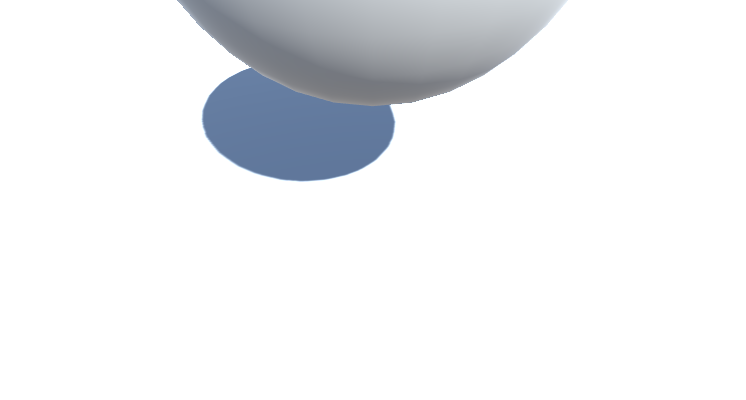
\includegraphics[width=\linewidth]{figures/shadows/directional-cleaned}
\caption{directional}
\label{fig:directional}
\end{subfigure}%
    \hfill
\begin{subfigure}[t]{0.33\textwidth}
\centering
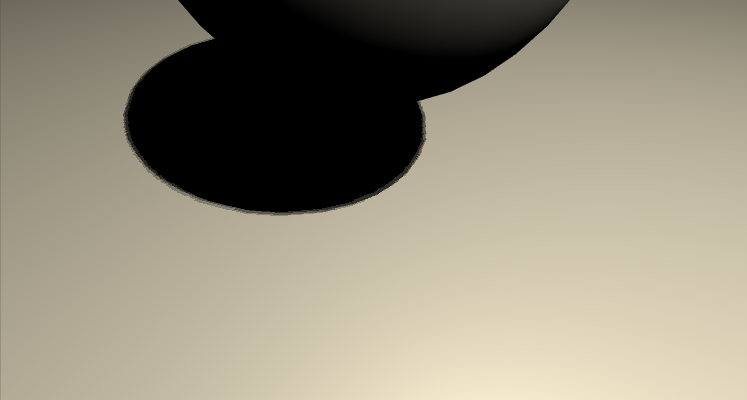
\includegraphics[width=\linewidth]{figures/shadows/point-cleaned}
\caption{point}
\label{fig:point}
\end{subfigure}%
    \hfill
\begin{subfigure}[t]{0.33\textwidth}
\centering

\includegraphics[width=\linewidth]{figures/shadows/point-far-cleaned}
\caption{point far}
\label{fig:point-far}
\end{subfigure}%

\caption{
(a) directional
(b) point
(c) point far
.}
\label{fig:rest-analysis}
\end{figure}


\begin{table}
  \centering
  \begin{tabular}{| c | c | c | c | }
    \hline
    & Narrow & Wide & Widest \\ \hline
    Close&  \begin{minipage}{.3\textwidth}
            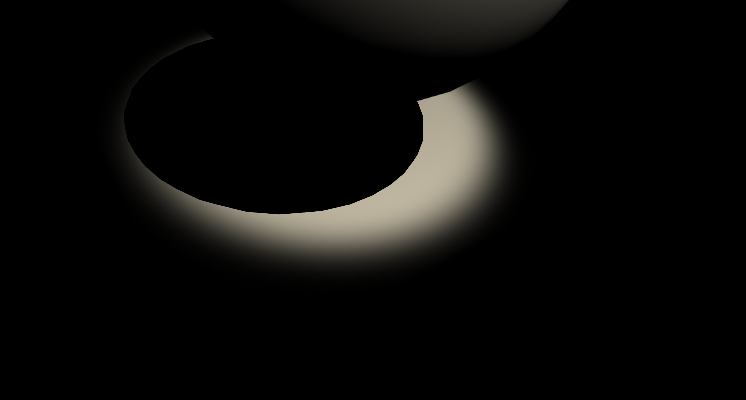
\includegraphics[width=\linewidth]{figures/shadows/spot-cleaned}
            \end{minipage}
            &
            \begin{minipage}{.3\textwidth}
            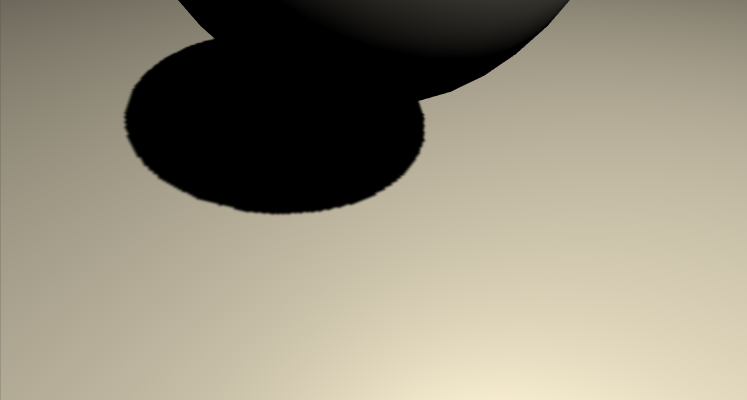
\includegraphics[width=\linewidth]{figures/shadows/spot-wide-cleaned}
            \end{minipage}
            & 
            \begin{minipage}{.3\textwidth}
            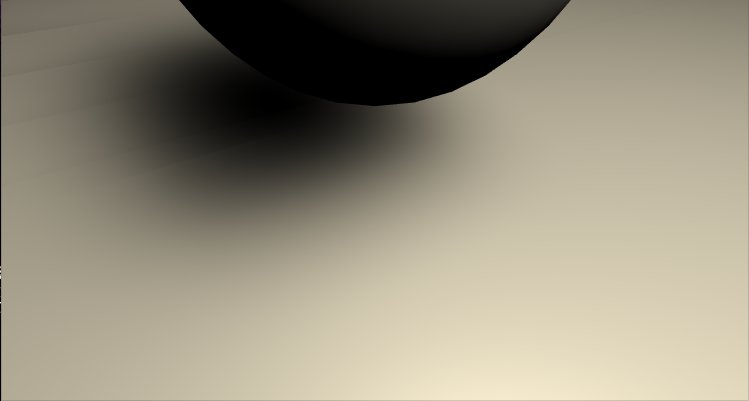
\includegraphics[width=\linewidth]{figures/shadows/spot-widest-cleaned}
            \end{minipage}
    \\ \hline
    Far &   \begin{minipage}{.3\textwidth}
            
\includegraphics[width=\linewidth]{figures/shadows/spot-far-cleaned}
            \end{minipage}
        &
            \begin{minipage}{.3\textwidth}
            
\includegraphics[width=\linewidth]{figures/shadows/spot-wide-far-cleaned}
            \end{minipage}
            & 
            \begin{minipage}{.3\textwidth}
            
\includegraphics[width=\linewidth]{figures/shadows/spot-widest-far-cleaned}
            \end{minipage}
    \\ \hline
  \end{tabular}
  \caption{Spot light analysis}\label{tbl:spot-analysis}
\end{table}

\section{Future Work}

\subsubsection{Refiner}
Recent advances in the computer vision field such as \cite{applerefiner}, tries to cope the approximations and limitations of simulations used to generate synthetic data sets. \cite{applerefiner} shows that using generative techniques that they can generate more realistic looking data from examples generated in a simulation. Such efforts can similarly be beneficial in this project, possibly adjusting shadows slightly to reflect a more realistic setting. 

\subsubsection{Effective Grasp Labelling}
As of now the only to way to tell the gripper in the simulation how to grasp any object, is to actually label each individual grasp manually for each object. This is quite a daunting task and not very interesting from a machine learning perspective, much rather an automatic way of labelling or detecting possible valid grasp would be beneficial to reach has higher degree of generality of the gripper simulations and thereby also the generated data sets

\bibliography{references}
\nocite{*} 

\begin{appendices}
%\renewcommand{\thesection}{\appendixname~\Alph{section}}
%\chapter{Appendix}
\renewcommand{\thesection}{\Alph{section}}
\section{Simulation}\label{app:simulation}


\includegraphics[width=\linewidth]{figures/simulation/depth-grabbing}
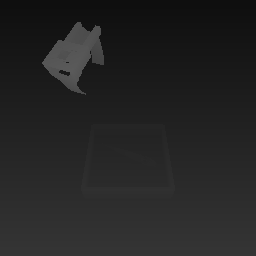
\includegraphics[width=\linewidth]{figures/simulation/depth-in}
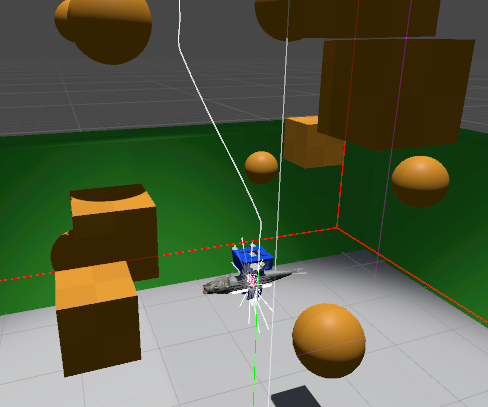
\includegraphics[width=\linewidth]{figures/simulation/editor-back}
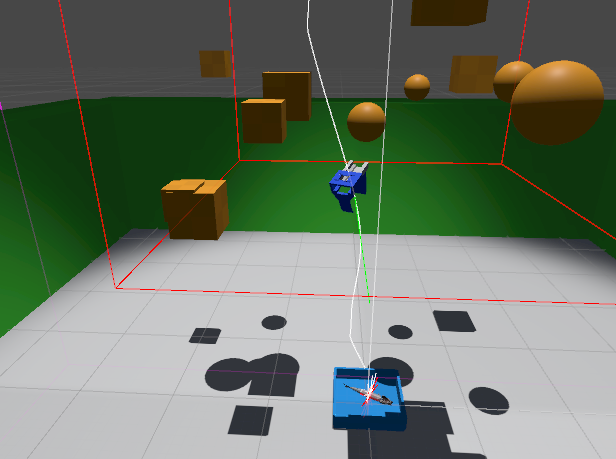
\includegraphics[width=\linewidth]{figures/simulation/editor-mid}
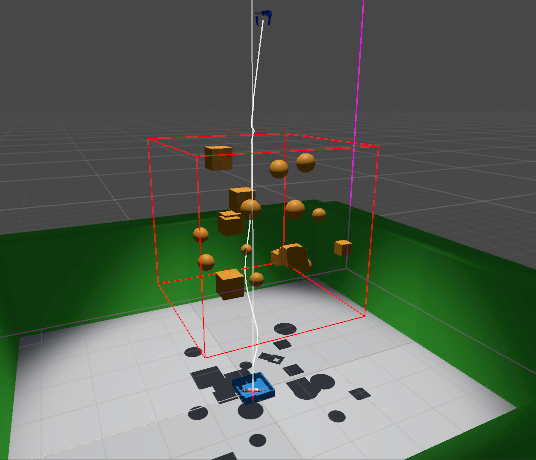
\includegraphics[width=\linewidth]{figures/simulation/editor}
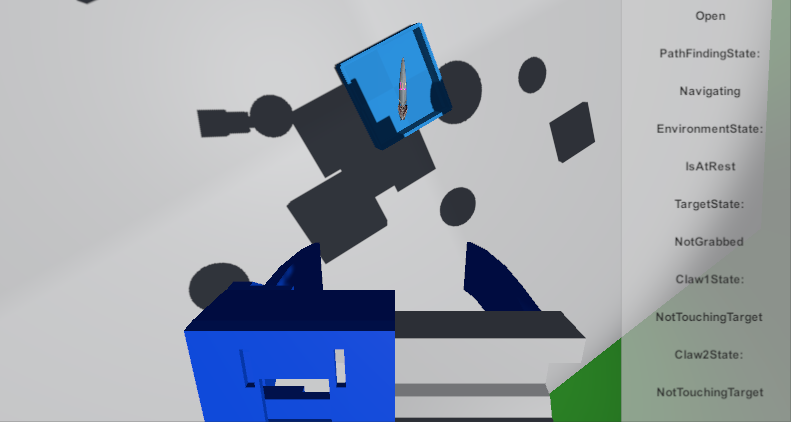
\includegraphics[width=\linewidth]{figures/simulation/game-mid}
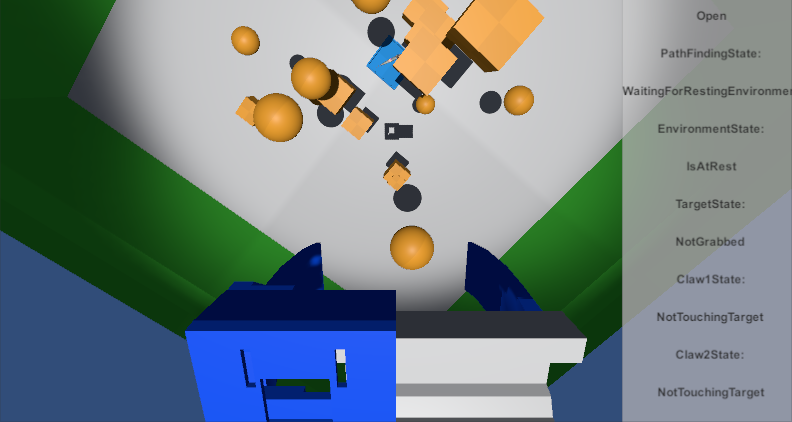
\includegraphics[width=\linewidth]{figures/simulation/game-start}
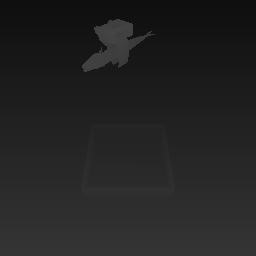
\includegraphics[width=\linewidth]{figures/simulation/grabbed-depth}
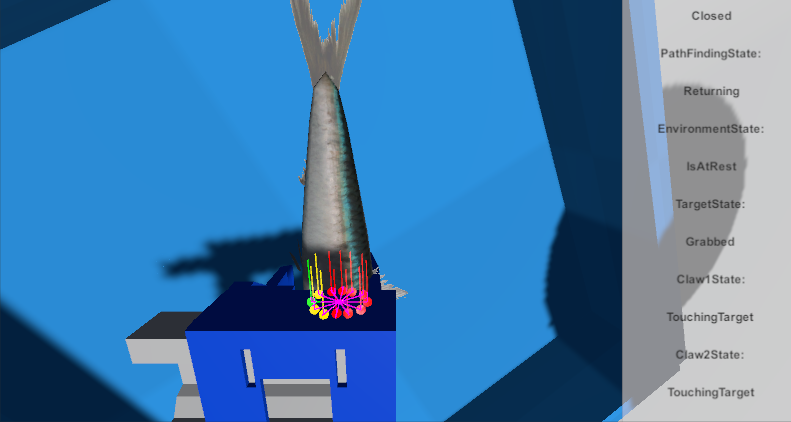
\includegraphics[width=\linewidth]{figures/simulation/grabbed}
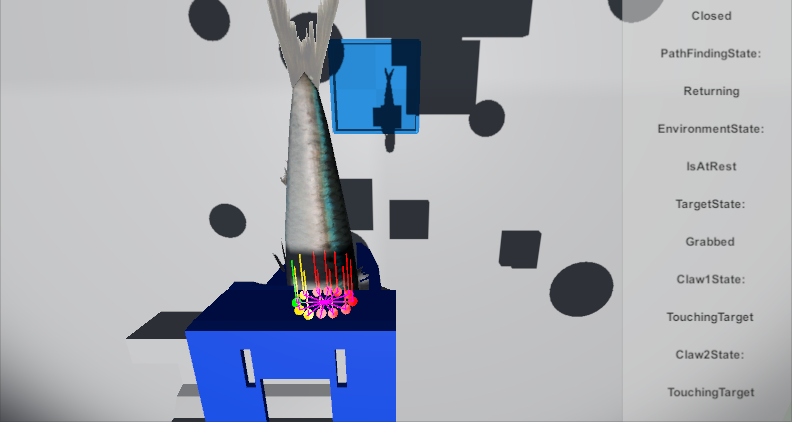
\includegraphics[width=\linewidth]{figures/simulation/returning}
\end{appendices}

\end{document}
